% !TeX program = xelatex
% Based on paper.hwp (submitted RE_v6); editable layout approximation.
% Duplicate introduction sentence removed; Accuracy@5 rounded to 65.55 from 449/685.
% Compile from this directory: xelatex paper.tex (twice).
\documentclass[a4paper,9pt,twocolumn]{extarticle}
\usepackage[left=18mm,right=18mm,top=15mm,bottom=15mm,headsep=8mm,footskip=8mm,columnsep=7mm]{geometry}
\usepackage{fontspec}
\usepackage{kotex}
\setmainfont{Times New Roman}
\setmainhangulfont{UnBatang}
\setsanshangulfont{Apple SD Gothic Neo}
\usepackage{titlesec}
\titleformat{\section}{\sffamily\bfseries\fontsize{11}{14.3}\selectfont}{\thesection.}{0.7em}{}
\titleformat{\subsection}{\bfseries\fontsize{9}{11.7}\selectfont}{\thesubsection}{0.7em}{}
\titlespacing*{\section}{0pt}{18pt}{9pt}
\titlespacing*{\subsection}{0pt}{9pt}{9pt}
\usepackage{graphicx,booktabs,tabularx,array,amsmath}
\usepackage{caption}
\usepackage{float}
\usepackage{placeins}
\usepackage{needspace}
\usepackage{xcolor}
\usepackage[hidelinks,breaklinks]{hyperref}
\usepackage{xurl}
\urlstyle{same}
\renewcommand{\figurename}{그림}
\renewcommand{\tablename}{표}
\renewcommand{\refname}{참고문헌}
\setlength{\parindent}{1em}
\setlength{\parskip}{2pt}
\renewcommand{\normalsize}{\fontsize{9}{11.7}\selectfont}
\normalsize
\emergencystretch=2em
\raggedbottom
\DeclareCaptionFont{kiiscaption}{\fontsize{8.5}{11.05}\selectfont}
\captionsetup{font=kiiscaption,labelfont=bf,labelsep=period,justification=centering}
\captionsetup[table]{position=top,skip=6pt}
\captionsetup[figure]{position=bottom,skip=6pt}
\begin{document}
\twocolumn[\begin{@twocolumnfalse}
\begin{center}
{\sffamily\fontsize{16}{20.8}\selectfont\bfseries 수학 문제 자동 해결을 위한 LLM-Lean 접근과 아키텍처 제안}\par\vspace{5pt}
{\sffamily\fontsize{12}{15.6}\selectfont Proposal of an LLM-Lean Approach and Architecture for Math Problem Solving}\par\vspace{8pt}
{\sffamily\fontsize{10}{13}\selectfont 이영직\textsuperscript{*} · 백재현\textsuperscript{**} · 정우석\textsuperscript{***} · 김범수\textsuperscript{***} · 김종락\textsuperscript{****}\textsuperscript{\dag}}\par
{\fontsize{10}{13}\selectfont Young Jik Lee, Jae-Hyun Baek, Woo-Seok Jeong, BeomSoo Kim, and Jon-Lark Kim\textsuperscript{\dag}}\par\vspace{5pt}
{\fontsize{10}{13}\selectfont *서강대학교 대학원 인공지능학과 석사과정, **서강대학교 대학원 인공지능학과 박사과정, ***서강대학교 대학원 수학과  석사과정, **** 서강대학교 대학원 수학과  교수\par
*MS Course, Department of Artificial Intelligence, Graduate School, Sogang University\par**Ph.D Course, Department of Artificial Intelligence, Graduate School, Sogang University\par*** MS Course, Department of Mathematics, Graduate School, Sogang University\par****Professor, Department of Mathematics \& Institute for Mathematical and Data Sciences, Sogang University \& DeepFountain Corp.}
\end{center}
\vspace{5pt}
\begingroup\fontsize{8.5}{11.05}\selectfont
\noindent{\sffamily\fontsize{11}{14.3}\selectfont\bfseries 요약}\par
본 연구는 명제의 참·거짓이 사전에 주어지지 않는 ‘Prove or disprove’ 문제를 대상으로 Single과 Dual Agent 구조의 문제 해결 성능을 비교한다. Single은 Prove와 Disprove 중 하나를 선택하여 증명하도록 하고, Dual은 탐색 방향을 선택하지 않고 두 경로를 병렬적으로 탐색하고 선택하는 구조이다. 최종 판정은 Lean 검증 결과에 따른다. 137개 문제의 Pass@5 평가에서 Single은 106개, Dual은 109개를 해결하였다. 두 구조는 문제 해결 성능이 유사하지만 코드 길이와 자원 사용에서 차이를 보였다.
\par\noindent\textbf{키워드 : AI4Math, 대규모 언어 모델, Lean, 자동 정리 증명}
\vspace{5pt}
\par\noindent{\sffamily\fontsize{11}{14.3}\selectfont\bfseries Abstract}\par
This study compares the problem-solving performance of Single and Dual agent architectures using “Prove or Disprove” problems in which the truth values of the propositions are not provided in advance. In the Single architecture, the agent selects either Prove or Disprove and attempts to prove the selected goal. In contrast, the Dual architecture explores both paths in parallel without selecting a single search direction. Final decisions are based on Lean verification results. In the Pass@5 evaluation of 137 problems, Single solved 106 problems, while Dual solved 109 problems. The two architectures demonstrated similar problem-solving performance but differed in generated code length and computational resource usage.
\par\noindent\textbf{Key Words : AI4Math, LLM, Lean, Automated Theorem Proving}
\par\endgroup
\vspace{8pt}
\end{@twocolumnfalse}]
\begingroup\renewcommand{\thefootnote}{}\footnotetext{\noindent\textsuperscript{\dag}Corresponding author: \href{mailto:jlkim@sogang.ac.kr}{jlkim@sogang.ac.kr}\par
본 연구는 National Natural Science Foundation of China, 과제번호 12471490의 지원을 받아 수행되었습니다. 또한 본 연구는 교육부와 한국연구재단이 재원으로 하는 4단계 BK21 사업(BK21 FOUR, Fostering Outstanding Universities for Research, 과제번호 4120240415042)의 부분적인 지원을 받아 수행되었습니다.
}\endgroup
% Template publication fields retained here for review, not treated as actual publication metadata:
% JKIIS
% 1976-9172
% 2288-2324
% ISSN(Print)
% ISSN(Online)
% Received: Jan. 01, 2015
% Revised : Jan. 01, 2015
% Accepted: Jan. 01, 2015
% This is an Open-Access article distributed under the terms of the Creative Commons Attribution Commercial License (http://creativecommons.org/licenses/by-nc/3.0) which permits unrestricted non-commercial use, distribution, and reproduction in any medium, provided the original work is properly cited.
% Journal of Korean Institute of Intelligent Systems
% Vol. 25, No. 3, June 2015, pp. 000-000
% http://dx.doi.org/10.5391/JKIIS.2015.25.3.000
\section{서론}


Lean 은 수학적 명제와 증명을 코드로 작성하고, 그 증명이 논리적으로 올바른지 기계적으로 확인하는 증명 보조기이다 \cite{r1}. Mathlib 는 이 과정에서 활용할 수 있는 수학적 정의와 정리들을 제공한다\cite{r2}. 최근에는 LLM을 활용하여 수학 문제와 증명을 Lean으로 자동 형식화 하는 연구가 진행되고 있으며, 형식화의 대상과 규모도 확대되고 있다\cite{r3,r4}. 또한 Lean은 주어진 명제뿐 아니라 그 부정에 대한 증명도 검증할 수 있다.
 수학 서적의 ‘Prove or Disprove’ 유형 문제는 명제의 참·거짓이 사전에 주어지지 않으므로, Prove와 Disprove 중 어느 방향으로 문제를 해결할 것인지 판단해야 한다. 이러한 문제에서는 Prove와 Disprove를 수행하는 능력뿐 아니라, 두 방향을 어떠한 방식으로 탐색할 것인지도 고려해야 한다. 본 연구에서는 이러한 문제를 대상으로, Prove와 Disprove 중 하나의 골(Goal)을 선택하여 탐색하는 Single(단일) 구조와 두 골을 동시에 탐색하는 Dual(이중) 구조를 비교한다. Single 구조에서는 Orchestrator가 매 라운드 Prove 또는 Disprove 중 하나의 골을 선택하고, 자신이 수행한 탐색 기록을 바탕으로 다음 전략을 수립한다. 반면, Dual 구조에서는 두 골을 별도의 경로에서 병렬로 탐색하며, Prove와 Disprove 경로의 기록을 함께 활용하여 후속 전략을 수립한다. 두 구조 모두 생성된 Lean 코드의 검증 결과를 바탕으로 최종 판정을 수행한다. 본 연구에서는 두 구조의 해결 성능, 생성 코드 길이 및 계산 비용을 비교하여 탐색 방식에 따른 성능과 효율성의 차이를 분석한다.
본 논문의 구성은 다음과 같다. 2장에서는 관련 연구를 검토하고, 3장에서는 데이터셋과 평가 조건을 설명한다. 4장에서는 Single 과 Dual 구조 및 Lean 판정 과정을 제시한다. 5장에서는 실험 결과를 분석하며, 6장에서는 결론과 향후 연구 방향을 논의한다. 에이전트별 상세 프롬프트와 실행 코드 및 데이터는 다음 공개 저장소에서 제공한다:
\url{https://github.com/lee-young-jik/Proposal-of-an-LLM-Lean-Approach-and-Architecture-for-Math-Problem-Solving.git}

\section{관련 연구}


수학적 추론에 Lean을 활용하는 연구에서는 명제를 증명하는 것뿐 아니라, 주어진 주장에 반증하고 그 결과를 검증하는 방법도 연구되고 있다.
HERMES \cite{r5}는 수학 문제의 풀이 과정에서 생성된 중간 주장을 Lean 명제로 변환하고, 해당 명제와 그 부정에 대한 증명을 병렬로 시도한다. 검증 결과를 이후 추론에 전달하여 풀이를 이어가거나 수정하며, 이전에 검증된 내용을 메모리에 저장하여 후속 추론에 활용한다. 이는 증명과 반증을 함께 탐색하여 풀이 과정에서 생성된 중간 주장의 타당성을 확인하는 접근이다.
AutoForm4Lean \cite{r6}은 조합론 문제를 생성하고 Lean으로 형식화하는 과정에서 Falsifier를 활용한다. Falsifier는 생성된 문제에 반례가 존재하는지 탐색하여 성립하지 않는 문제를 걸러낸다. 이 연구에서 반증은 생성된 문제의 품질을 점검하는 역할을 한다.
Learning to Disprove \cite{r7}는 수학적 명제에 대한 반례와 그 타당성을 뒷받침하는 Lean 증명을 함께 생성하도록 LLM을 학습한다. 반례를 자연어로 제시하는 데 그치지 않고, 형식적으로 검증할 수 있는 반증을 생성하는 데 초점을 둔다.
Lean Disprove\cite{r8}는 수학적 명제에 대한 반례를 탐색하고 이를 Lean 으로 검증하는 도구를 제안한다. 값의 열거, 탐색 범위 확장 및 외부 도구를 활용하여 반례를 찾으며, 최종적으로 Lean에서 검증된 반증만을 인정한다.
기존 연구에서는 중간 추론의 타당성 검증, 생성된 문제의 선별 및 반례 탐색을 위해 증명과 반증을 활용하였다. 반면 본 연구는 참·거짓이 사전에 알려지지 않은 명제를 해결하는 과정에서, 증명과 반증 중 하나를 선택하는 Single 구조와 두 방향을 병렬로 탐색하는 Dual 구조의 차이를 분석한다. 또한 두 구조의 탐색 기록 활용 방식과 탐색 예산을 명시하고, 동일한 Lean 검증 기준에 따라 해결 성능, 생성 코드 길이 및 계산 비용을 비교한다.

\section{데이터셋 및 평가 예산}


본 연구에서는 고등학교에서 대학교 수준의 수학 서적을 대상으로, Prove와 Disprove 중 어느 방향으로 해결해야 하는지 사전에 알려지지 않은 문제를 총 137개 수집하였다. 본 절에서는 데이터셋의 구축 과정과 Single 및 Dual 구조의 비교를 위한 평가 예산을 설명한다.

\subsection{사용 데이터}


본 연구에서는 공개된 고등학교에서 대학교 수준의 수학 관련 서적 5권에서 Prove 또는 Disprove 여부가 사전에 알려지지 않은 “Prove or Disprove” 유형의 문제를 총 137개 수집하였다. Hammack의 Book of Proof (edition 3.4)\cite{r9}에서는 기초증명·집합·관계·함수, Lebl의 Basic Analysis I (version 6.3) \cite{r10}에서는 실해석학, Axler 의 Linear Algebra Done Right (4 판)\cite{r11}에서는 선형대수학, Erdman 의 Exercises and Problems in Calculus\cite{r12}에서는 미적분학, Judson 의 Abstract Algebra: Theory and Applications\cite{r13}에서는 추상대수학 문제를 가져왔다. Prove 문제는 62개, Disprove 문제는 75개이다. 서적별 문제 수와 정답 분포는 표 1에 제시하였다.


\begin{center}

\captionof{table}{서적별 문제 수와 정답 분포\\Table \thetable. Problem Counts and Labels by Textbook}
\label{tab:book_sources}
\footnotesize
\setlength{\tabcolsep}{3pt}\renewcommand{\arraystretch}{1.15}
\begin{tabularx}{\columnwidth}{>{\raggedright\arraybackslash}Xrrr}
\toprule
Textbook & Prove & Disprove & Total \\
\midrule
Book of Proof \cite{r9} & 24 & 31 & 55 \\
Basic Analysis I \cite{r10} & 2 & 11 & 13 \\
Linear Algebra Done Right \cite{r11} & 6 & 20 & 26 \\
Exercises and Problems in Calculus \cite{r12} & 8 & 13 & 21 \\
Abstract Algebra: Theory and Applications \cite{r13} & 22 & 0 & 22 \\
\midrule
\textbf{Total} & \textbf{62} & \textbf{75} & \textbf{137} \\
\bottomrule
\end{tabularx}
\end{center}

\subsection{정답 Lean 데이터셋 구축 방법}


본 연구에서는 고등학교에서 대학교 수준의 수학 관련 서적 5권에서 137개 문제를 Lean으로 검증할 수 있는 형태로 변환하였다. 데이터 구축에는 gpt-6.1-sol을 사용하였으며, 각 문제에 대해 원래 명제를 증명하는 Prove 골과 그 명제가 성립하지 않음을 증명하는 Disprove 골을 각각 생성하였다. 이후 사람이 직접 검수하여 생성된 Lean 골이 원래 수학 문제의 의미와 일치하는지 확인하였다. 이를 통해 하나의 문제에서 Prove와 Disprove 모두 시도할 수 있도록 하였다. 예를 들어, “모든 실수 \(x,y\)에 대해 \(|x+y|=|x|+|y|\)가 성립하는지 Prove하거나 Disprove하라”는 문제를 생각할 수 있다. Prove 골은 해당 등식이 모든 실수에서 성립함을 증명하는 것이고, Disprove 골은 등식이 성립하지 않는 경우가 존재함을 증명하는 것이다. 실제로 \(x=1,\ y=-1\)일 때 왼쪽은 0, 오른쪽은 2이므로 등식이 성립하지 않는다. 따라서 이 문제의 올바른 해결 방향은 Disprove이다. 정답 데이터는 각 문제의 올바른 해결 방향에 해당하는 Lean 증명 코드를 작성하고, 실제 Lean 검증을 통과하는지 확인하여 구축하였다. 정답 코드는 원래의 골을 유지하고 sorry와 axiom을 사용하지 않는 형태로 작성하였다. 최종 데이터셋은 Prove 문제 62개와 Disprove 문제 75개로 구성하였다. 실제 실험에서는 Orchestrator에 자연어 문제와 Prove·Disprove 골을 모두 제공하되, 정답 방향과 정답 코드는 알려주지 않았다. 정답 방향은 문제 해결 여부를 평가하는 데 사용하고, 정답 코드는 시스템이 생성한 코드의 길이를 비교하는 기준으로 활용하였다.

\subsection{평가 예산}


본 연구에서는 탐색 예산을 라운드(Round)와 시도(Trial) 라는 두 단위로 정의한다. 라운드는 Orchestrator 가 Lean 증명 전략을 수립하는 단위이고, 시도는 해당 Lean 증명 전략과 자연어 증명을 바탕으로 Lean 코드를 생성하고 검증하는 과정이다. 각 라운드 에서는 경로별로 전략과 자연어 증명을 한 번씩 생성하며, Lean 코드의 생성 및 검증 기회를 최초 시도 1회와 오류 수정 후 재시도 2회를 합하여 최대 3회 부여한다. 재시도 에서는 같은 전략과 자연어 증명을 유지하고, Repair Agent의 수정 지침을 반영하여 Lean 코드를 수정한다. Single은 선택한 한 경로에서 최대 3회, Dual은 Prove와 Disprove의 각 경로에서 최대 3회씩 시도한다. 어느 한 골이라도 검증을 통과하면 종료하며, 해당 라운드의 모든 시도가 실패하면 이전 탐색 기록을 바탕으로 새로운 Lean 증명 전략을 수립하여 다음 라운드로 넘어간다. 라운드는 최대 3 회까지 수행하며, 최대 3라운드의 전체 탐색을 독립적으로 5회 반복하였으며, 구체적인 값은 표 2와 같다.

\begin{table}[htbp]\centering\footnotesize
\caption{에이전트 예산\\Table \thetable. Agent Budget}\label{tab:1}
\setlength{\tabcolsep}{3pt}\renewcommand{\arraystretch}{1.2}
\begin{tabularx}{\columnwidth}{>{\raggedright\arraybackslash}p{.43\columnwidth}XX}
\toprule
Item & Single & Dual \\
\midrule
Metric & \textnormal{Pass@5} & \textnormal{Pass@5} \\
Max strategy rounds & 3 & 3 \\
\textnormal{Max trials per round} & \textnormal{3} & \textnormal{3+3} \\
Model-call timeout & 900s & 900s \\
Lean verification timeout & 300s & 300s \\
\bottomrule\end{tabularx}\end{table}

\section{제안 아키텍처}


본 장에서는 제안하는 시스템의 구조를 설명한다. 제안 시스템 은 하나의 Orchestrator 와 여러 서브 에이전트로 이루어진 다중 에이전트 구조이다. Orchestrator가 Lean 증명 전략을 세우면, 서브 에이전트들이 자연어 증명을 제안하고 이를 Lean 코드로 옮긴 뒤 검증한다. 이처럼 계획을 담당하는 역할과 실행을 담당하는 역할을 분리하는 구조는 최근 연구에서도 제안된 바 있다\cite{r14,r15}. 본 연구에서는 매 라운드 Prove 골과 Disprove 골 중 하나를 선택하여 증명을 시도하는 Single 구조와, 두 골을 별도의 경로에서 병렬로 탐색하는 Dual 구조를 비교한다. Dual 구조의 Prove 경로와 Disprove 경로는 각각 배정된 골의 증명을 시도한다. 에이전트별 사용 모델 은 표 3과 같다.

\begin{table}[htbp]\centering\footnotesize
\caption{에이전트별 사용모델\\Table \thetable. Model assigned to each agent}\label{tab:2}
\setlength{\tabcolsep}{3pt}\renewcommand{\arraystretch}{1.2}
\begin{tabularx}{\columnwidth}{>{\raggedright\arraybackslash}p{.35\columnwidth}X}
\toprule
\textnormal{Model} & \textnormal{Agents} \\
\midrule
\textnormal{gpt-6-luna-pro} & \textnormal{Orchestrator} \\
\textnormal{gpt-6-luna} & \textnormal{Natural Agent, Lean Generator, Repair Agent} \\
\bottomrule\end{tabularx}\end{table}

\begin{figure*}[t]\centering
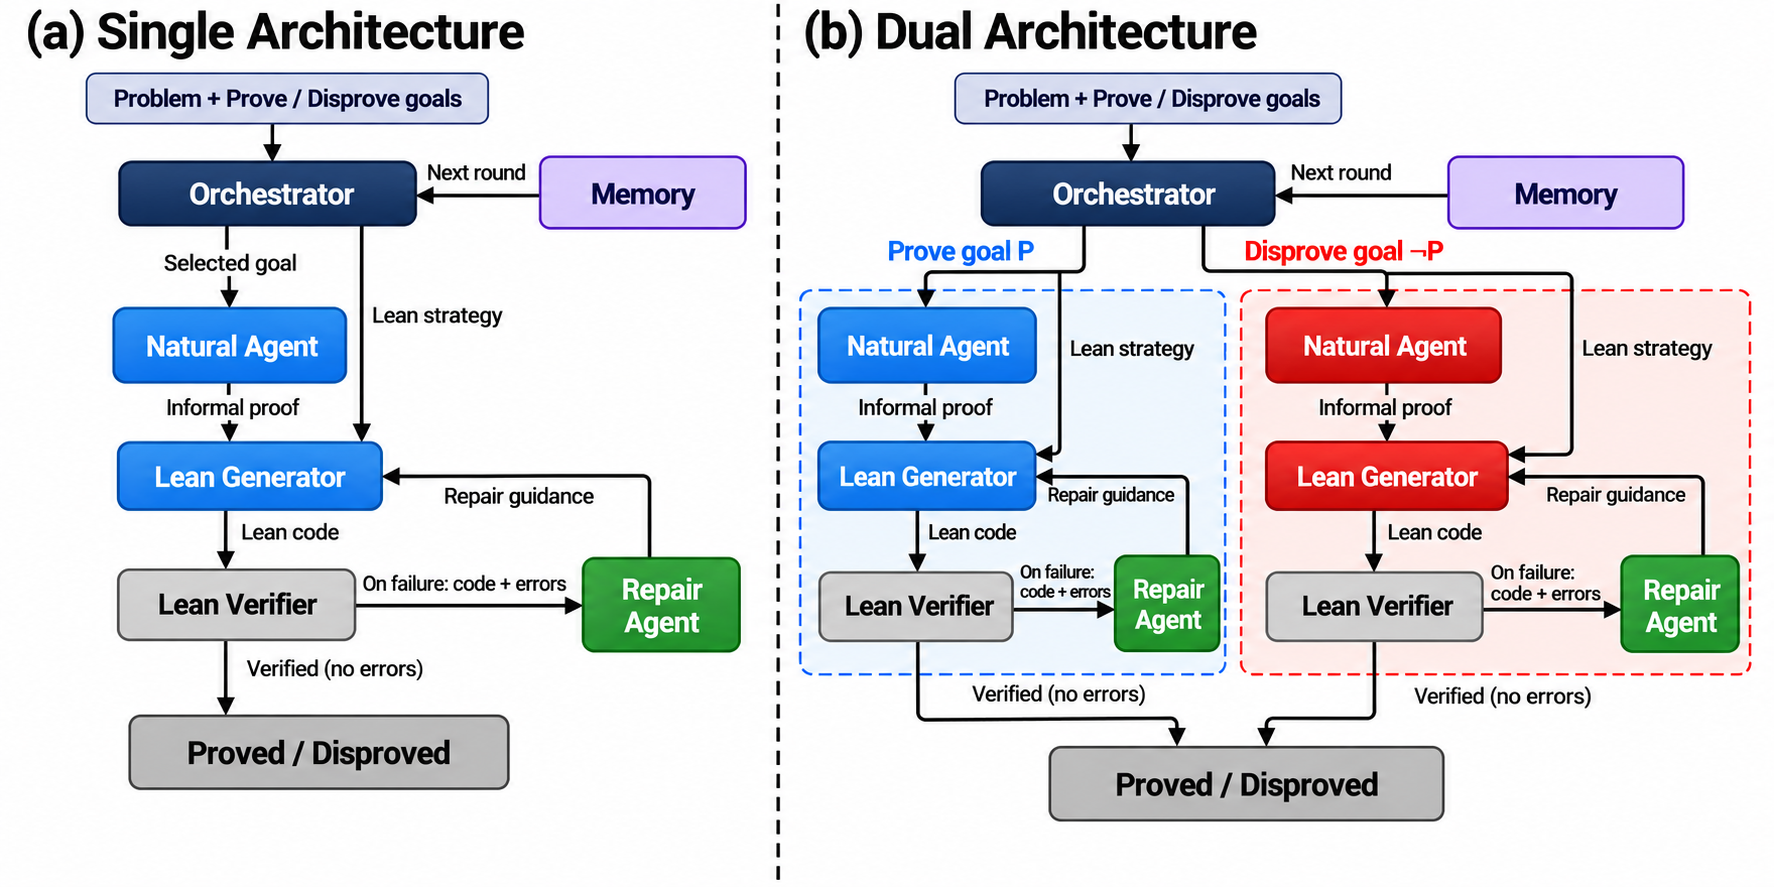
\includegraphics[width=\textwidth,height=.68\textheight,keepaspectratio]{assets/figure1_architecture.png}
\caption{(a) Single 구조 (b) Dual 구조\\Fig. \thefigure. (a) Single Architecture (b) Dual Architecture}\label{fig:1}\end{figure*}

\subsection{Single(단일) 구조}


Single 구조의 전체 흐름은 그림 1(a)에 제시하였다. Single 구조에서는 Orchestrator에 문제와 함께 Prove 골과 Disprove 골을 모두 제공한다. Orchestrator는 문제를 검토하여 두 골 중 하나를 선택하고, 선택한 골을 해결하기 위한 Lean 증명 전략을 수립한다. 이 과정에서 문제의 정답 유형과 정답 코드는 제공하지 않는다. Natural Agent는 문제와 선택된 골을 바탕으로 자연어 증명을 작성한다. Lean Generator는 선택된 골, Orchestrator의 Lean 증명 전략 및 Natural Agent 의 자연어 증명을 활용하여 Lean 코드를 생성한다. 생성된 코드가 Lean 검증에 실패하면 Repair Agent가 골, 전략, 자연어 증명, 생성된 코드 및 Lean 오류 메시지를 참고하여 Lean 코드 수정 지침을 작성한다. Lean Generator는 직전 코드와 오류 메시지, 수정 지침을 바탕으로 코드를 다시 생성한다. 이때 같은 라운드의 자연어 증명은 유지한다. 한 라운드에서는 최대 3 회의 Lean 검증을 시도한다. 모두 실패하면 해당 라운드의 전략, 자연어 증명 및 생성된 코드를 메모리에 저장한다. 다음 라운드에서 Orchestrator는 이전 탐색 기록을 참고하여 Prove 골과 Disprove 골 중 하나를 다시 선택하고, 선택한 골에 맞는 Lean 증명 전략을 새롭게 수립한다. 이때 이전 라운드와 동일한 골을 선택하거나 다른 골로 전환할 수 있다. 이러한 과정을 최대 3 라운드까지 반복하며, 어느 골도 Lean 검증을 통과하지 못하면 Unsolved로 처리한다.



\subsection{Dual(이중) 구조}


Dual 구조의 전체 흐름은 그림 1(b)에 제시하였다. Dual 구조에서는 Orchestrator가 Prove 골과 Disprove 골에 대한 전략을 각각 수립한다. Single 에서는 두 골 중 하나를 선택하지만, Dual에서는 두 골을 모두 탐색하도록 각 경로의 전략을 세운다. Prove 경로는 원명제의 증명을, Disprove 경로는 원명제의 부정에 대한 증명을 동시에 시도하며, 탐색 중에도 각 경로의 골은 유지된다. 이 과정에서 문제의 정답 유형과 정답 코드 는 제공하지 않는다. Natural Agent는 문제와 해당 경로의 골을 바탕으로 자연어 증명을 작성한다. Lean Generator는 해당 골, Orchestrator 가 수립한 전략 및 자연어 증명을 활용하여 Lean 코드를 생성한다. 두 경로는 이러한 과정을 각각 수행한다. 생성된 코드가 Lean 검증에 실패하면 Repair Agent가 골, 전략, 자연어 증명, 생성된 코드 및 Lean 오류 메시지를 참고하여 수정 지침을 작성한다. Lean Generator는 직전 코드와 오류 메시지, 수정 지침을 바탕으로 코드를 다시 생성한다. 이때 같은 라운드의 자연어 증명은 유지한다. 한 라운드에서는 경로별로 최대 3회의 Lean 검증을 시도한다. 두 경로 모두 실패하면 각 경로의 전략, 자연어 증명 및 생성된 코드를 메모리에 저장한다. 다음 라운드에서 Orchestrator 는 양쪽 경로의 이전 탐색 기록을 함께 참고하여 Prove 경로와 Disprove 경로의 전략을 각각 다시 수립한다. 이때 두 경로의 골은 그대로 유지하고, 각 골을 해결하기 위한 Lean 증명 전략을 새롭게 세운다. 참고하는 기록은 이전 라운드까지 누적된 내용이며, 같은 라운드에서 생성 중인 기록은 두 경로 사이에 공유하지 않는다. 어느 한 경로에서 Lean 검증에 성공하면 해당 결과에 따라 판정을 확정하고 다른 경로의 추가 탐색을 종료한다. 이러한 과정을 최대 3라운드까지 반복하며, 어느 골도 Lean 검증을 통과하지 못하면 Unsolved로 처리한다.

\subsection{Lean 검증 및 결과 판정}


본 연구에서는 생성된 Lean 코드의 검증 결과로 최종 판정을 내린다. 검증 과정에서는 원래 Lean 골의 변경과 추가 선언을 제한하고, sorry, admit, axiom 등의 사용을 금지한다. 각 문제에는 원 명제 \(P\)를 증명하는 Prove 골과 그 부정 \(\neg P\) 를 증명하는 Disprove 골을 제공한다. Natural Agent 의 자연어 증명은 코드 생성을 돕는 정보로 사용하며, 최종 판정의 근거로 사용하지 않는다. Prove 골의 증명이 Lean 검증을 통과하면 Proved, Disprove 골의 증명이 검증을 통과하면 Disproved로 판정한다. 정해진 탐색 예산 내에 어느 골도 해결하지 못하면 Unsolved 로 처리한다. 한쪽 골을 증명하지 못했다는 이유만으로 반대쪽 판정을 내리지는 않는다. 이 판정 기준은 Single 과 Dual 에 동일하게 적용한다. 성능 평가에서는 Prove 문제를 Proved로, Disprove 문제를 Disproved 로 판정한 경우를 정답으로 집계한다.

\subsection{메모리 구조}


메모리는 이전 라운드의 탐색 기록을 다음 전략 수립에 활용하기 위한 장치이다. Orchestrator에 전달하는 메모리는 라운드와 탐색 방향별로 묶이며, 각 묶음에는 (1) Lean 증명 전략(strategy), (2) 자연어 증명(informal proof), (3) 각 시도의 Lean 코드가 포함된다. Single은 각 라운드에서 선택한 Prove 또는 Disprove 방향의 기록을 누적하고, 다음 라운드의 Orchestrator 는 이전 라운드까지의 기록을 참고하여 골을 선택하고 Lean 증명 전략을 수립한다. Dual 은 같은 라운드 안에서는 두 경로의 기록을 공유하지 않고, 라운드가 끝나면 양쪽 기록을 Orchestrator에 전달하여 다음 전략 수립에 활용한다. 두 구조 모두 독립 반복 실행 사이에는 메모리를 공유하지 않는다. 두 구조의 Orchestrator 메모리는 그림 2에 나타냈다.

\begin{figure}[htbp]\centering
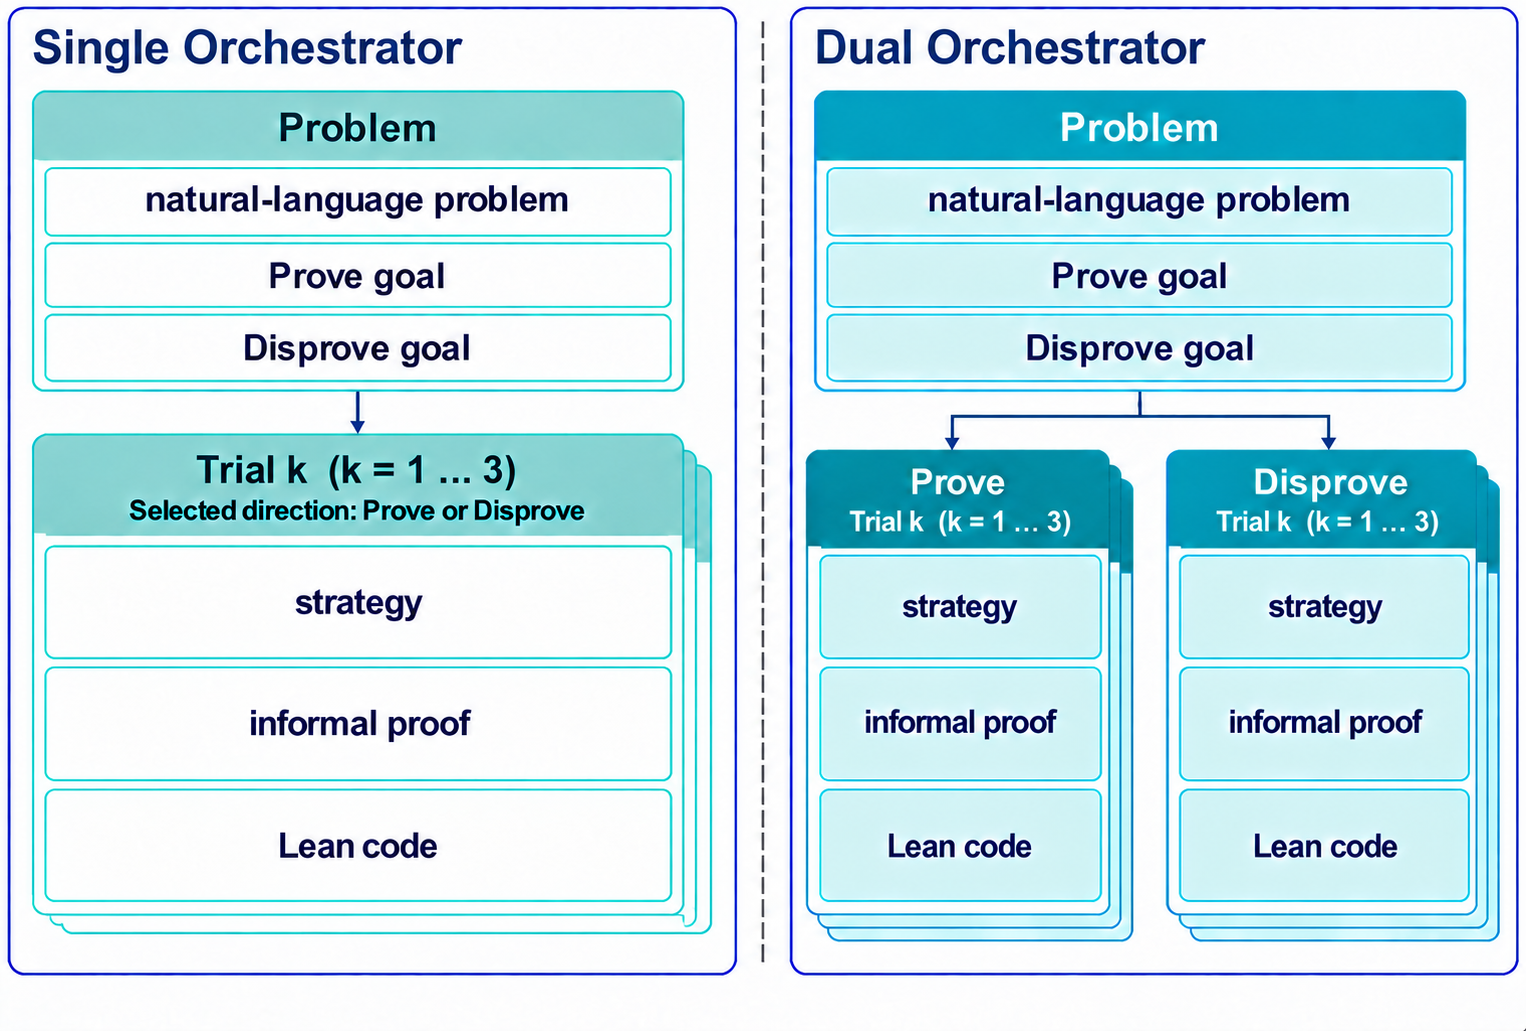
\includegraphics[width=\columnwidth,keepaspectratio]{assets/figure2_memory.png}
\caption{(a) 단일 구조 메모리 (b) 이중 구조 메모리\\Fig. \thefigure. (a) Single memory (b) Dual memory}\label{fig:2}\end{figure}

\FloatBarrier
\section{실험 및 결과}


\subsection{문제 해결 결과}


전체 137개 문제는 Prove 62개와 Disprove 75개로 구성된다. Pass@5 평가 결과, Single은 Proved 50개, Disproved 56개, Unsolved 31개로 총 106개(77.37\%)를 해결하였으며, Dual은 Proved 52개, Disproved 57개, Unsolved 28개로 총 109개(79.56\%)를 해결하였다. Accuracy@5는 5회 독립 실행에서 각 실행의 정답률을 평균한 지표로, Single은 62.77\%, Dual은 65.55\%로 나타났다. 두 구조의 평가 결과는 표 4에 제시하였다. 두 구조가 공통으로 해결한 문제는 106개였으며, Single만 해결한 문제는 없고 Dual만 해결한 문제는 3개였다. 또한 5회 반복 실행에서 실행당 평균 해결 문제 수는 Single 86.0 ± 2.45개, Dual 89.8 ± 1.30개로 나타났다. 하지만 두 구조의 Pass@5 기준 문제별 해결 여부에 대해 양측 정확 McNemar 검정을 수행한 결과, 통계적으로 유의한 차이는 확인되지 않았다(p = 0.25).

\begin{table}[htbp]\centering\footnotesize
\caption{전체 137개 문제에 대한 Pass@5 및 Accuracy@5 평가 결과\\Table \thetable. Pass@5 and Accuracy@5 Results on 137 Problems}\label{tab:3}
\setlength{\tabcolsep}{3pt}\renewcommand{\arraystretch}{1.2}
\begin{tabularx}{\columnwidth}{>{\raggedright\arraybackslash}Xccc}
\toprule
Architecture & P/D/U & Pass@5 (\%) & Accuracy@5 (\%) \\
\midrule
Single & 50/56/31 & 77.37 & 62.77 \\
Dual & 52/57/28 & 79.56 & 65.55 \\
\bottomrule
\end{tabularx}
\par\vspace{3pt}\begin{minipage}{\columnwidth}\footnotesize
P/D/U는 Proved/Disproved/Unsolved 문제 수이다. Pass@5는 5회 중 한 번이라도 해결한 문제 수를 137로 나눈 비율이며, Accuracy@5는 전체 정답 실행 수를 \(137\times5=685\)로 나눈 비율이다.
\end{minipage}
\end{table}

\subsection{정답 대비 생성 코드 길이 비교 }


3.2절에서 구축한 정답 Lean 데이터셋의 코드 길이를 기준으로 문제를 짧은 코드, 중간 길이 코드, 긴 코드의 세 구간으로 구분하였다. 표 5는 각 구간의 Pass@5 결과와 생성 코드의 정답 대비 평균 길이 배수인 Length Ratio를 나타낸다. Length Ratio는 5회 반복 실행에서 각 문제에 대해 최초로 정답 판정을 받은 생성 코드의 길이를 정답 데이터셋의 Lean 코드 길이로 나눈 값으로 정의하였다. 분석 결과, 평균 Length Ratio는 모든 구간에서 Dual이 Single보다 낮게 나타났다. 짧은 코드 구간에서는 Single 4.91배, Dual 4.75배였으며, 중간 길이 구간에서는 각각 2.30배와 2.08배, 긴 코드 구간에서는 1.48배와 1.32배였다. 각 구조가 해결한 전체 문제에서도 Single은 3.18배, Dual은 2.96배로 나타났다. 이는 Dual이 정답 코드 대비 평균적으로 더 짧은 성공 코드를 생성하는 경향을 보여준다.


\begin{table}[htbp]\centering\footnotesize
\caption{코드 길이 구간별 Pass@5 및 생성 코드 길이 배수\\Table \thetable. Pass@5 and Generated Code Length Ratios by Code Length Group}\label{tab:4}
\setlength{\tabcolsep}{2pt}\renewcommand{\arraystretch}{1.25}
\begin{tabularx}{\columnwidth}{l*{4}{>{\centering\arraybackslash}X}}
\toprule
 & \multicolumn{2}{c}{Single} & \multicolumn{2}{c}{Dual} \\
\cmidrule(lr){2-3}\cmidrule(lr){4-5}
Group & Pass@5 & Length ratio & Pass@5 & Length ratio \\
\midrule
Short & 44/46 & 4.91 & 44/46 & 4.75 \\
Medium & 36/46 & 2.30 & 37/46 & 2.08 \\
Long & 26/45 & 1.48 & 28/45 & 1.32 \\
\midrule
Overall & 106/137 & 3.18 & 109/137 & 2.96 \\
\bottomrule
\end{tabularx}

\end{table}

\subsection{메모리 활용에 따른 문제 해결 결과}


첫 라운드에서 Orchestrator는 이전 탐색 기록 없이 문제와 골을 바탕으로 전략을 수립한다. 해당 라운드의 모든 시도가 Lean 검증에 실패하면 사용한 전략, 자연어 증명 및 Lean 코드를 메모리에 저장한다. 이후 2·3라운드에서는 이전 탐색 기록을 참고하여 Lean 증명 전략을 다시 수립하고 문제 해결을 시도한다. 표 6은 각 문제의 5회 반복 실행 중 처음 성공한 실행을 기준으로, 해당 실행에서 문제가 해결된 라운드를 집계한 결과이다. 첫 라운드에서 Single은 66개, Dual은 77개 문제를 해결하였다. 첫 라운드에서 해결하지 못한 문제 중 이전 탐색 기록을 활용해 전략을 다시 수립한 2·3라운드에서는 Single이 40개, Dual이 32개 문제를 추가로 해결하였다. 이는 두 구조 모두 이전의 실패한 탐색 기록을 참고하여 전략을 재수립한 후 문제 해결에 성공한 사례가 있음을 보여준다. 특히 Dual은 첫 라운드에서 Single보다 11개 많은 문제를 해결하여 초기 탐색 단계에서 상대적으로 높은 문제 해결 성능을 보였다. 한편 Single에서는 후속 라운드에 실제 정답 유형과 다른 탐색 방향을 선택한 사례가 총 11회 관찰되었다. 이는 이전 탐색 기록을 활용하더라도 정답과 다른 방향을 선택하는 경우가 있음을 보여준다.

\begin{table}[htbp]\centering\footnotesize
\caption{메모리 활용에 따른 라운드별 문제 해결 수\\Table \thetable. Number of Problems Solved by Round Using Memory}\label{tab:memory}
\setlength{\tabcolsep}{4pt}\renewcommand{\arraystretch}{1.2}
\begin{tabularx}{\columnwidth}{>{\raggedright\arraybackslash}Xrrr}
\toprule
Architecture & Round 1 & Round 2 & Round 3 \\
\midrule
Single & 66 & 30 & 10 \\
Dual & 77 & 25 & 7 \\
\bottomrule
\end{tabularx}

\end{table}

\subsection{자원 사용량}


두 구조의 계산 자원 사용량을 비교하기 위해 입력 및 출력 토큰, 실행 시간과 API 비용을 분석하였다. 표 7은 137개 문제의 5회 반복 실행을 대상으로, 미해결 실행을 포함한 구조별 685회 실행의 평균값을 나타낸다. Dual의 평균 총 토큰 사용량은 Single의 약 1.86배, 실행 시간 은 약 1.23배, 기록된 API 비용은 약 1.75배였다. 따라서 앞서 관찰한 Dual의 작은 코드 길이 배수가 추론 과정의 자원 절감을 의미하지는 않으며, 유사한 정답률을 얻는 데 더 많은 자원이 사용되었다. 실행 시간은 실행 환경과 API 응답 지연의 영향을 포함한 관측값이다.

\begin{table}[htbp]\centering\footnotesize
\caption{문제당 1회 실행의 평균 자원 사용량\\Table \thetable. Mean Resource Usage per Problem Execution}\label{tab:resources}
\setlength{\tabcolsep}{4pt}\renewcommand{\arraystretch}{1.2}
\begin{tabularx}{\columnwidth}{>{\raggedright\arraybackslash}Xrr}
\toprule
Metric & Single & Dual \\
\midrule
Input tokens & 92,408 & 174,885 \\
Output tokens & 14,989 & 25,137 \\
Total tokens & 107,397 & 200,022 \\
Execution time (s) & 395.4 & 485.6 \\
API cost (USD) & 0.00873 & 0.01531 \\
\bottomrule
\end{tabularx}
\end{table}

\section{결론 및 향후 연구}


본 연구에서는 명제의 참·거짓이 사전에 주어지지 않는 고등학교에서 대학교 수준의 수학 관련 서적의 ‘Prove or Disprove’ 문제를 대상으로 Single과 Dual 구조의 탐색 방식과 문제 해결 성능을 비교하였다. Dual은 Single보다 근소하게 높은 해결 성능을 나타냈다. 또한 정답 코드 대비 생성 코드의 평균 길이 배수는 모든 길이 구간에서 Dual이 더 낮았다. 이는 두 구조의 문제 해결 성능이 유사하더라도 생성하는 코드의 길이에는 차이가 있을 수 있음을 보여준다. 메모리 활용에 따른 문제 해결 결과에서는 Dual이 첫 라운드에서 Single보다 많은 문제를 해결하여 초기 탐색 단계에서 상대적으로 높은 문제 해결 성능을 보이는 경향이 나타났다. 이후 이전 탐색 기록을 바탕으로 전략을 재수립한 2·3라운드에서는 두 구조 모두 추가 문제를 해결한 사례가 관찰되었다. 한편 Single에서는 후속 라운드에 실제 정답 유형과 다른 탐색 방향을 선택하는 사례도 관찰되었다. 자원 사용량 측면에서 Dual이 Prove와 Disprove를 동시에 탐색하므로 Single보다 많은 토큰을 사용하였으며, 실행 시간과 API 비용도 높게 나타났다. 특히 정답과 다른 탐색 경로에도 자원이 사용되어 추가적인 계산 비용이 발생할 수 있다. 따라서 Dual의 상대적으로 간결한 성공 코드와 추가적인 계산 비용을 함께 고려할 필요가 있다.
향후 연구에서는 Retrieval-Augmented Formalization을 활용하여 이전 탐색 기록을 보다 효율적으로 활용하는 방법을 연구하고자 한다. 현재 구조에서는 이전 라운드의 탐색 기록 전체를 Orchestrator에 제공하지만, 후속 연구에서는 문제와 관련성이 높은 기록을 선택적으로 검색하여 전략 수립과 Lean 코드 생성에 활용할 계획이다. 이를 통해 불필요한 정보 전달을 줄이고, 토큰 사용량과 실행 시간 및 API 비용을 효율적으로 관리하면서 문제 해결 성능을 유지하거나 개선할 수 있는 탐색 구조를 개발하고자 한다.
\FloatBarrier
\section*{Conflict of Interest}
저자는 본 논문에 관련된 어떠한 잠재적인 이해상충도 없음을 선언한다.
\begingroup\small
\begin{thebibliography}{99}
\bibitem{r1} L. de Moura and S. Ullrich, “The Lean 4 theorem prover and programming language,” Automated Deduction – CADE 28, Lecture Notes in Computer Science, vol. 12699, Springer, pp. 625-635, 2021, doi: 10.1007/978-3-030-79876-5\_37.

\bibitem{r2} The mathlib Community, “The Lean mathematical library,” Proceedings of the 9th ACM SIGPLAN International Conference on Certified Programs and Proofs (CPP 2020), New Orleans, LA, USA, pp. 367-381, Jan. 2020, doi: 10.1145/3372885.3373824.

\bibitem{r3} S. Lee et al., “Lean-GAP: A dataset of formalized graduate algebra problems,” arXiv preprint, arXiv:2606.02588, 2026.

\bibitem{r4} F. Gloeckle et al., “Automatic textbook formalization,” arXiv preprint, arXiv:2604.03071, 2026.

\bibitem{r5} A. Ospanov, Z. Feng, J. Sun, H. Bai, S. Xin, and F. Farnia, “HERMES: Towards efficient and verifiable mathematical reasoning in LLMs,” Proceedings of the 43rd International Conference on Machine Learning (ICML 2026), Proceedings of Machine Learning Research, vol. 306, Seoul, South Korea, pp. 94942-94966, Jul. 2026.

\bibitem{r6} L. Doan and T. Nguyen, “AI-assisted autoformalization of combinatorics problems in proof assistants,” Proceedings of the IEEE/ACM 47th International Conference on Software Engineering: New Ideas and Emerging Results (ICSE-NIER), Ottawa, Canada, pp. 1-5, Apr. 2025, doi: 10.1109/ICSE-NIER66352.2025.00006.

\bibitem{r7} Z. Li, Z. Li, K. Yang, X. Ma, and Z. Su, “Learning to disprove: Formal counterexample generation with large language models,” arXiv preprint, arXiv:2603.19514, 2026.

\bibitem{r8} J. Ondras and C. Freer, “Lean Disprove: Certified counterexample search for AI-assisted formal mathematics,” Proceedings of the 3rd AI for Math Workshop: Toward Self-Evolving Scientific Agents, ICML 2026, Seoul, South Korea, Jul. 2026. Available: \url{https://icml.cc/virtual/2026/82610}, [Accessed: October 22, 2026].

\bibitem{r9} R. Hammack, Book of Proof, ed. 3.4, 2025. Available: \url{https://richardhammack.github.io/BookOfProof/}, [Accessed: October 22, 2026].

\bibitem{r10} J.Lebl, Basic Analysis I: Introduction to Real Analysis, Volume I, ver. 6.3, 2026. Available: \url{https://www.jirka.org/ra/realanal.pdf}, [Accessed: October 22, 2026].

\bibitem{r11} S. Axler, Linear Algebra Done Right, 4th ed., Springer, 2024. Available: \url{https://linear.axler.net/}, [Accessed: October 22, 2026].

\bibitem{r12} J. M. Erdman, Exercises and Problems in Calculus, Portland State University, ver. Aug. 1, 2013. Available: \url{https://web.pdx.edu/~erdman/CALCULUS/CALCULUS\_pdf.pdf}, [Accessed: October 22, 2026].

\bibitem{r13} T. W. Judson, Abstract Algebra: Theory and Applications, 2026. Available: \url{https://judsonbooks.org/aata-files/aata-html/aata-toc.html}, [Accessed: October 22, 2026].

\bibitem{r14} H. Ju et al., “Automated conjecture resolution with formal verification,” arXiv preprint, arXiv:2604.03789, 2026.

\bibitem{r15} S. Varambally, T. Voice, Y. Sun, Z. Chen, R. Yu, and K. Ye, “Hilbert: Recursively building formal proofs with informal reasoning,” Proceedings of the International Conference on Learning Representations (ICLR 2026), Rio de Janeiro, Brazil, Apr. 2026.
\end{thebibliography}\endgroup
\section*{저자 소개}
\noindent\begin{minipage}{\columnwidth}
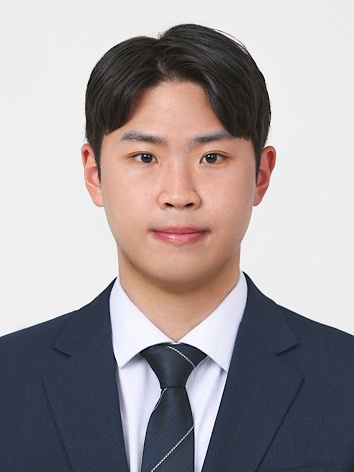
\includegraphics[width=20mm,height=25mm,keepaspectratio]{assets/author_lee.png}\hfill\begin{minipage}[b]{\dimexpr\columnwidth-24mm\relax}\textbf{이영직(Young Jik Lee)}\end{minipage}\par\smallskip
2023년:연세대학교 미래캠퍼스 컴퓨터공학과\par
공학사\par
2025년\textasciitilde{}현재:서강대학교 대학원\par
인공지능학과 석사과정\par
관심분야:LLM, AI Agent, AI4Math\par
ORCID Number : 0009-0000-6662-9061\par
E-mail: yjlee@sogang.ac.kr\par
\end{minipage}\par\vspace{12pt}

\noindent\begin{minipage}{\columnwidth}
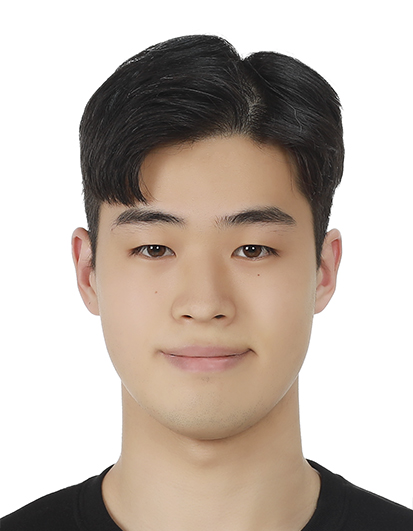
\includegraphics[width=20mm,height=25mm,keepaspectratio]{assets/author_baek.png}\hfill\begin{minipage}[b]{\dimexpr\columnwidth-24mm\relax}\textbf{백재현(Jae-Hyun Baek)}\end{minipage}\par\smallskip
2024년:서강대학교 수학과 이학사\par
2024년\textasciitilde{}2026년:서강대학교 대학원 수학과 데이터사이언스 전공 석사\par
2026년\textasciitilde{}현재:서강대학교 대학원\par
인공지능학과 박사과정\par
관심분야:LLM, deep learning, AI security\par
ORCID Number : 0009-0006-2765-636X\par
E-mail: jhbaek@sogang.ac.kr\par
\end{minipage}\par\vspace{12pt}

\noindent\begin{minipage}{\columnwidth}
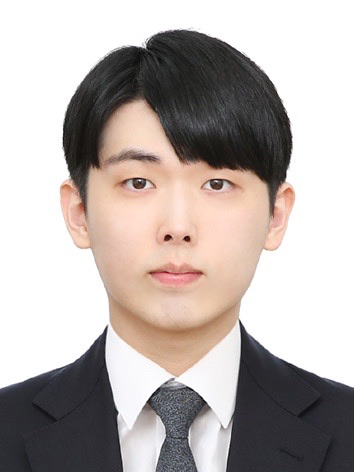
\includegraphics[width=20mm,height=25mm,keepaspectratio]{assets/author_jeong.png}\hfill\begin{minipage}[b]{\dimexpr\columnwidth-24mm\relax}\textbf{정우석(Woo-Seok Jeong)}\end{minipage}\par\smallskip
2025년:경기대학교 수학과 이학사\par
융합데이터공학부(복수전공)\par
통계학과(부전공)\par
2025년\textasciitilde{}현재:서강대학교 대학원 수학과\par
데이터사이언스 전공 석사과정\par
관심분야:LLM, RAG, AI Agent, AI4Math\par
ORCID Number : 0009-0003-5782-2523\par
E-mail: wsj0813@sogang.ac.kr\par
\end{minipage}\par\vspace{12pt}

\noindent\begin{minipage}{\columnwidth}
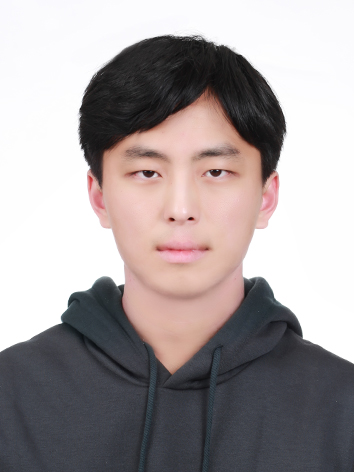
\includegraphics[width=20mm,height=25mm,keepaspectratio]{assets/author_kim_beomsoo.png}\hfill\begin{minipage}[b]{\dimexpr\columnwidth-24mm\relax}\textbf{김범수(BeomSoo Kim)}\end{minipage}\par\smallskip
2024년:서강대학교 수학과 이학사\par
2024년\textasciitilde{}2026년:서강대학교 대학원 수학과 데이터사이언스 전공 석사과정\par
관심분야:Reinforcement learning, Algebra\par
ORCID Number : 0009-0001-9614-9904\par
E-mail: cyclone.so.ga@gmail.com\par
\end{minipage}\par\vspace{12pt}

\noindent\begin{minipage}{\columnwidth}
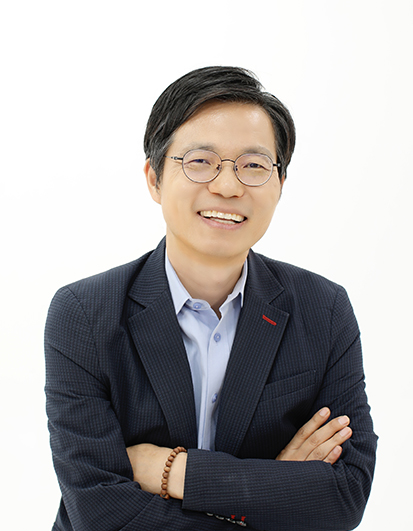
\includegraphics[width=20mm,height=25mm,keepaspectratio]{assets/author_kim_jonlark.png}\hfill\begin{minipage}[b]{\dimexpr\columnwidth-24mm\relax}\textbf{김종락(Jon-Lark Kim)}\end{minipage}\par\smallskip
1993년:포스텍 수학과 졸업\par
1997년:서울대학교 수학과 석사 졸업\par
2002년 : 일리노이 주립대학교 (시카고)\par
수학과 박사\par
2005\textasciitilde{}2012년 : 루이빌 대학교 조교수,\par
부교수\par
2012\textasciitilde{}현재 : 서강대학교 수학과 교수\par
관심분야:Coding Theory, Cryptography, Information Theory, Artificial Intelligence\par
ORCID Number : 0000-0002-0517-9359\par
E-mail        : jlkim@sogang.ac.kr\par
\end{minipage}\par\vspace{12pt}

\end{document}
